\section*{1}

Se considera el siguiente problema de optimización:
\begin{equation*}
\begin{aligned}
    (P) \quad \min \quad & 2 x_1 + x_2 \\
    \text{sujecto a} \quad & x_1^2 + x_2^2 \leq 4, \\
\end{aligned}
\end{equation*}

\begin{enumerate}[label=(\alph*)]
    \item Obtenga gráficamente la solución del problema (P).
    \item Obtenga el problema dual (D) de (P). 
    \item Resuelva el problema dual (D) obtenido y demuestre que los valores óptimos de (P) y (D) coinciden.
\end{enumerate}

\noindent\rule{10cm}{0.4pt}

\subsection*{(a)}

El problema tiene un minimo en $\left(-\frac{4}{\sqrt{5}}, -\frac{2}{\sqrt{5}}\right)$, como se ve en la figura.
\begin{figure}[h]
\centering
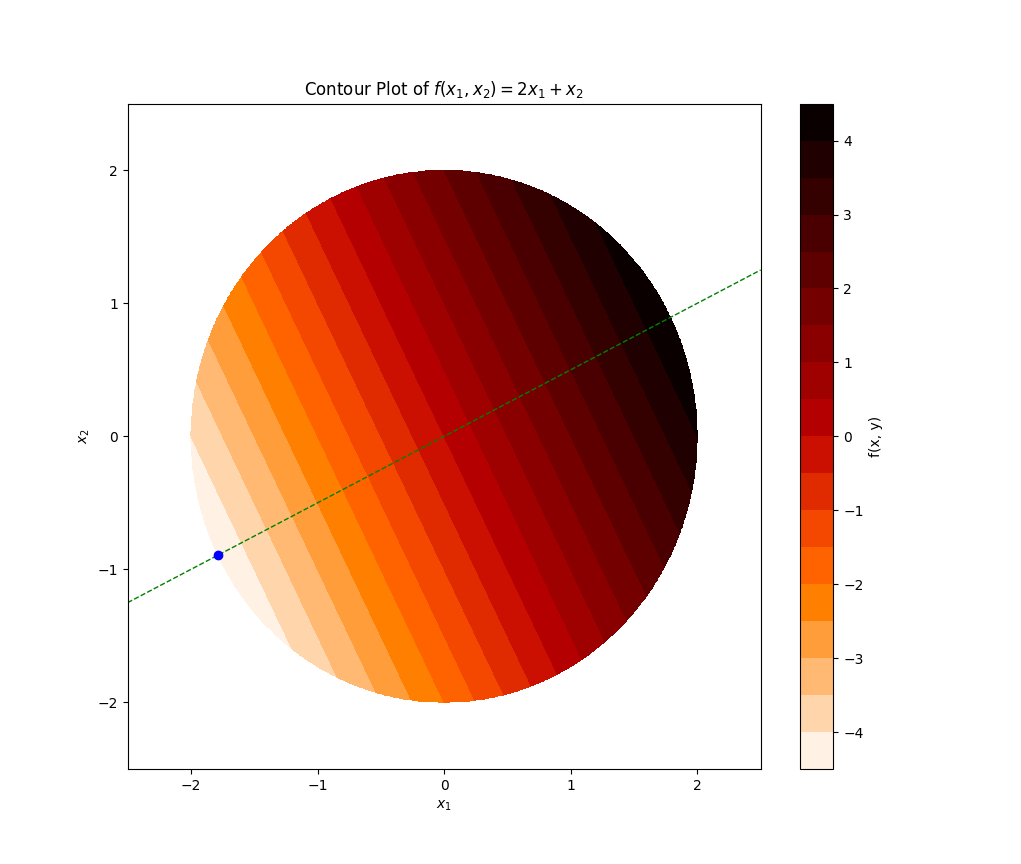
\includegraphics[scale=0.6]{ex1_solution.png}
\caption{Solución gráfica del problema.}
\label{ex1_solution}
\end{figure}

\subsection*{(b)}

El problema dual de $(P)$ se puede escribir como
\begin{equation*}
    \max_{u \geq 0} \inf_{(x_1, x_2) \in \R^2} 2 x_1 + x_2 + u ( x_1^2 + x_2^2 - 4 ).
\end{equation*}


\subsection*{(c)}

En el caso en que $x_1^2 + x_2^2 > 4$ entonces cuando $u \rightarrow \infty$ el valor del problema tiende a $\infty$,
si $x_1^2 + x_2^2 \leq 4$ entonces el máximo se alcanza cuando $u = 0$.
Por tanto el problema dual es equivalente al primal
\begin{equation*}
\begin{aligned}
    (D) \quad \inf \quad & 2 x_1 + x_2 \\
    \text{sujecto a} \quad & x_1^2 + x_2^2 \leq 4, \\
\end{aligned}
\end{equation*}
y sus valores óptimos coinciden.

Para encontrar el valor optimo,
planteamos el sistema de condiciones KKT
\begin{equation*}
\begin{aligned}
    2 + 2 u_1 x_1 & = 0, \\
    2 + 2 u_1 x_2 & = 0, \\
    x_1^2 + x_2^2 - 4 & = 0, \\
    u_1 \geq 0,
\end{aligned}
\end{equation*}
de la primera ecuacion tenemos que $x_1 = -\frac{1}{u_1}$ de la segunda $x_2 = -\frac{1}{2 u_1}$,
substituyendo en la tercera igualdad
\begin{equation*}
    \frac{1}{u_1^2} + \frac{1}{4 u_1^2} - 4 = 0
    \Rightarrow u_1 = \frac{\sqrt{5}}{4},
\end{equation*}
por tanto $\left( -\frac{4}{\sqrt{5}}, -\frac{2}{\sqrt{5}} \right)$ es un mínimo del problema,
como la función $f(x_1, x_2) = 2 x_1 + x_2$ es afín y la función $g_1(x_1, x_2) = x_1^2 + x_2^2 - 4$ es convexa,
por el Teorema 5.17 del libro de texto $\left( -\frac{4}{\sqrt{5}}, -\frac{2}{\sqrt{5}} \right)$ es solución del problema con valor $-\frac{10}{\sqrt{5}}$.
